% ------------------
% -- Assignment 1 --
% -- Math 4171 -----

\documentclass[6pt,oneside]{article}

%\usepackage{subfigure}
\usepackage{subcaption}
\usepackage{graphicx}
\usepackage{amsmath}
\usepackage{amsfonts}
\usepackage{hyperref}
\usepackage{adjustbox}
\usepackage{listings}
\usepackage{xcolor}
\usepackage{titlesec}
\usepackage{enumitem}
\usepackage{mathrsfs}
\usepackage{anyfontsize}
\usepackage[driver=pdftex]{geometry}
\usepackage{import}
\usepackage{cleveref}
\usepackage{multicol}

%\usepackage{titleformat{\section
%        {\normalfont\normalzie\bfseries}{Helo.}{1em}{}


\definecolor{codegreen}{rgb}{0,0.6,0}
\definecolor{codegray}{rgb}{0.5,0.5,0.5}
\definecolor{codepurple}{rgb}{0.58,0,0.82}
\definecolor{backcolour}{rgb}{0.95,0.95,0.92}
 
\lstdefinestyle{mystyle}{
    backgroundcolor=\color{backcolour},   
    commentstyle=\color{codegreen},
    keywordstyle=\color{magenta},
    numberstyle=\tiny\color{codegray},
    stringstyle=\color{codepurple},
    basicstyle=\fontsize{8}{10}\selectfont\ttfamily,
    breakatwhitespace=false,         
    breaklines=true,                 
    captionpos=b,                    
    keepspaces=true,                 
    numbers=left,                    
    numbersep=5pt,                  
    showspaces=false,                
    showstringspaces=false,
    showtabs=false,                  
    tabsize=2
}
\lstset{style=mystyle}

\newtheorem{theorem}{Theorem}
\newtheorem{definition}{Definition}
\newtheorem{proof}{Proof}
 

%\usepackage[margin=0.5in]{geometry}
%\usepackage{inputenc}

\newcommand{\Real}{\mathbb{R}}
\newcommand{\Int}{\mathbb{Z}}
\newcommand{\Nat}{\mathbb{N}}
\newcommand{\Complex}{\mathbb{C}}
\newcommand{\vect}[1]{\boldsymbol{#1}}

\renewcommand{\Re}[1]{\mathfrak{Re}\left\lbrace{#1}\right\rbrace}
\renewcommand{\Im}[1]{\mathfrak{Im}\left\lbrace{#1}\right\rbrace}

\title{{\bf Squeeze-Excitation Networks\\An easy to implement attention mechanism}\\\vspace{10pt}     
    \author{Jacques Nel}
}

\begin{document}

\maketitle

\section{Introduction}

The convolutional operator, used in CNNs, has an essentially local receptive field.
Recently, there have been some spectacular results achieved by neural network architectures that rely
on attention mechanisms. The transformer, for example, consists entirely of an attention mechanism,
and manages to achieve state-of-the-art results on NLP tasks.\footnote{Vaswani et al., "Attention Is All You Need", NIPS 2017.}

The \emph{Squeeze-and-Excitation (SE)} block allows the model to model complex inter-channel dynamics, and
allows a global flow of information, similar to an attention mechanism.\footnote{Hu et al., "Squeeze-and-Excitation Networks".}
SE blocks are simple to implement, and can simply be added to any pre-existing model architecture. SE
blocks can significantly improve a model's performance, at a marginal additional computational cost.

\section{SE architecture}

The SE block is build around a convolutional operator. Let
$\vect{X}\in\Real^{H'\times W' \times C'}$ denote the input signal, with height, width, and channel depth being $H', W',$ and $C'$
respectively.

$$
\vect{F}_{tr} : \vect{X} \in \Real^{H'\times W'\times C'}\rightarrow \vect{U}\in\Real^{H\times W\times C}
$$

Take $\vect{F}_{tr}$ to be a convolutional operator with learned filter kernels
$\vect{V}=\left[ \vect{v}_1, \ldots, \vect{v}_C\right]$. In other words

$$
\vect{u}_c = \vect{v}_c \ast \vect{X} = \sum_{s=1}^{C'} \vect{v}_c^s \ast \vect{x}^s.
$$

\begin{figure}[h]
    \center
    \caption{Squeeze-and-Excitation architecture}
    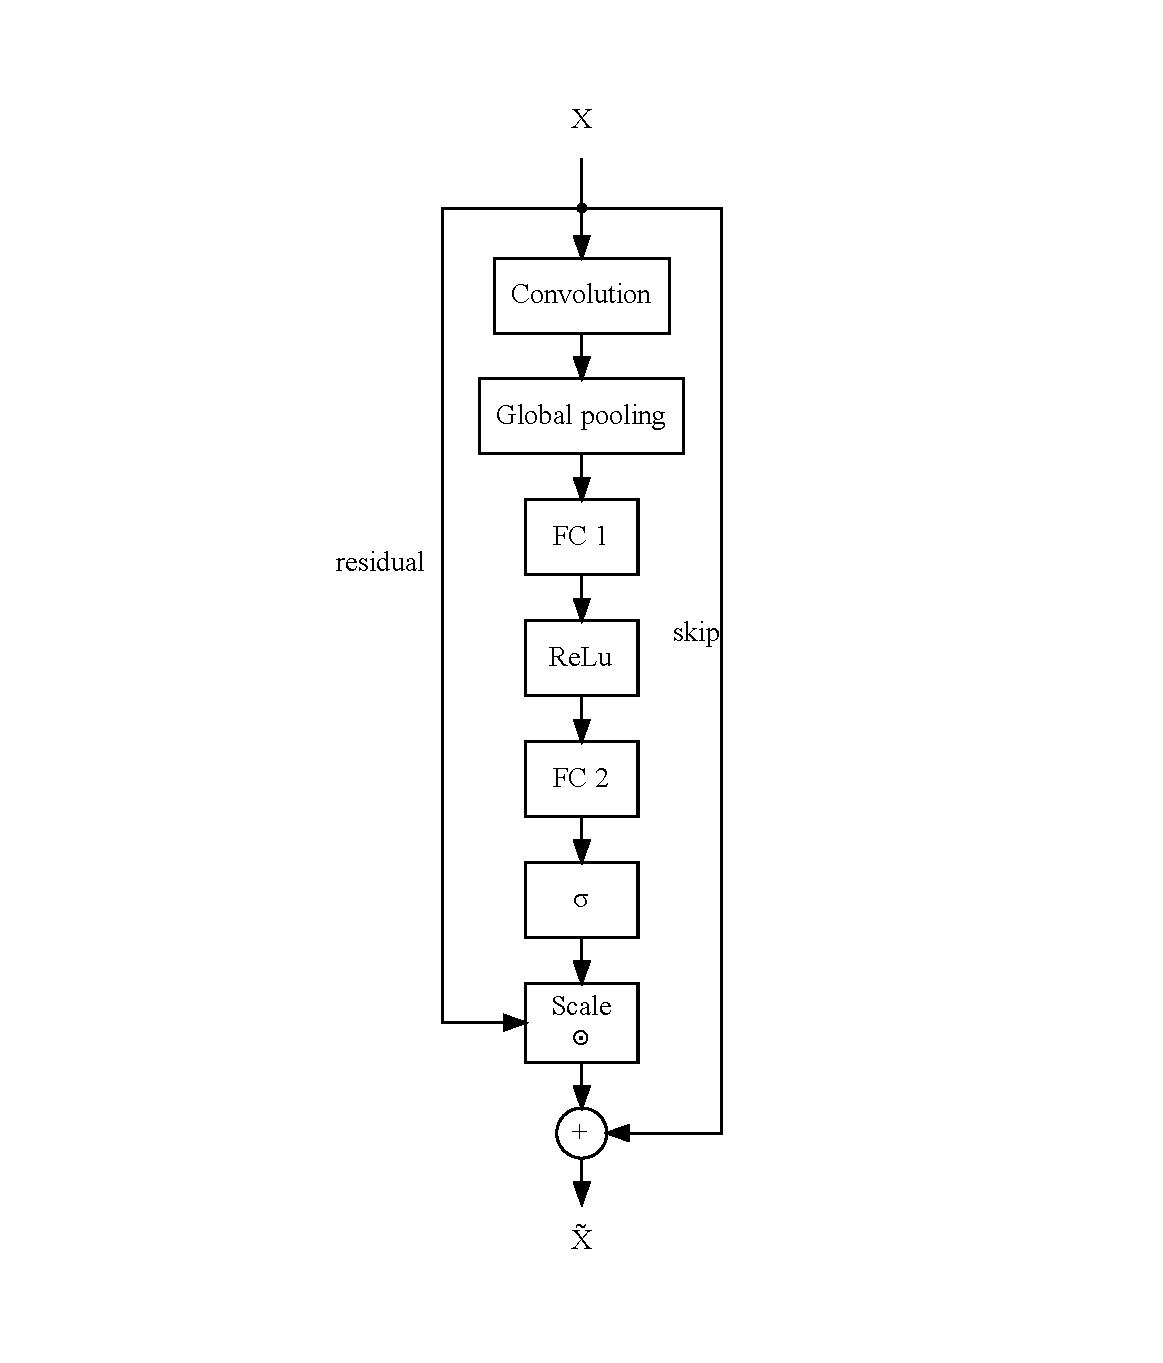
\includegraphics[scale=0.6]{se}
\end{figure}

\subsection{Squeeze operation}

Each filter map operates with a local receptive field and can not utilize information outside of its region.
First, a global channel statistic is generated by a \emph{squeeze} operation, consisting of an average 
pooling layer.

$$
z_c = \vect{F}_{sq}(\vect{u}_c) = \frac{1}{HC}\sum_{i=1}^H\sum_{j=1}^W u_c(i, j).
$$

\subsubsection{Excitation}

Next, an \emph{excitation} layer allows channel-wise dependence to be learned on the output of the
\emph{squeeze} operation. This simply consists of a simple gating mechanism with two fully connected
layers, a sigmoid, and ReLu activation function.

$$
\vect{s} = \vect{F}_{ex}(\vect{z}, \vect{W}_1, \vect{W}_2)
=
\sigma( \vect{W}_2\mathrm{ReLu}(\vect{W}_1\vect{z})),
$$

where $\vect{W}_1 \in \Real^{\frac{C}{\rho}\times C}$ and $\vect{W}_2 \in \Real^{C\times\frac{C}{\rho}}$.
The reduction ratio $\rho$, preferably a divisor of $C$, allows one to control the number of parameters.
The \emph{excitation} operator acts as a bottleneck. In effect, the SE block acts as a self-attention
mechanism, acting on a wider domain than the receptive field of the individual convolution filters.

Finally, the output of the SE block is produced by scaling $\vect{U}$ with the signal $\vect{s}$.

$$
\tilde{\vect{x}}_c = \vect{F}_{scale}(\vect{u}_c, s_c) = s_c\vect{u}_c.
$$

We also use a skip connection, that bypasses the SE block entirely.

\newpage

\section{Implementation}

The idea of an SE block is extremely simple to implement.

\begin{lstlisting}[language=Python]
import torch
import torch.nn as nn
import torch.nn.functional as F
from torch.optim import Adam
from torch.utils.data.dataloader import DataLoader


class SeBlock2d(nn.Module):

    def __init__(self,
                 channels, 
                 ratio=2):

        super().__init__()

        self.conv = nn.Conv2d(in_channels=channels, 
                              out_channels=channels,
                              kernel_size=3,
                              padding=1)

        self.gate_1 = nn.Linear(in_features=channels,
                                out_features=channels // ratio)
        self.gate_2 = nn.Linear(in_features=channels // ratio,
                                out_features=channels)

    def forward(self, x):

        # Generate feature maps U.
        u = self.conv(x)
        h, w = x.shape[-2:]

        # Apply global average pooling to calculate channel descriptor z.
        z = 1. / (h + w) * torch.sum(u, dim=(-2, -1))

        # Pass signal through two fully connected layers of excitation operator.
        s = torch.sigmoid(self.gate_2(F.relu(self.gate_1(z))))
        s = s.unsqueeze(-1).unsqueeze(-1)

        # Scale by activation s.
        x_out = s * u

        return x_out

\end{lstlisting}

\end{document}
